\documentclass[arbeit=studie, oneside, BCOR=12mm]{ArbeitRST}
% Die Option BCOR legt den Rand für die Bindekorrektur links fest
% (verschiebt das ganze Dokument nach rechts auf dem Papier, damit
% Platz zum Binden ist
\usepackage{enumitem}
\usepackage{graphicx}
\usepackage{float}
% bib-Datei mit den Literaturangaben
% Nutzung von biber/biblatex, Erläuterungen
% siehe Text!
% =========================================
\addbibresource{SA_Rockstroh_Literatur.bib}

% Zwei Parameter zum Verändern des Layouts
% ========================================
% \parindent -> Legt fest, mit welcher Einrückung jeder neue
%               Absatz beginnen soll
% \parskip -> Legt fest, wieviel vertikaler Abstand zwischen zwei
%             Absätzen liegen soll
%
% Tipp: Entweder parindent auf Null und parskip auf einen Wert
% ungleich Null (z.B. 2ex) oder umgekehrt. Beide Werte ungleich
% Null macht satztechnisch keinen Sinn. 1ex = Breite des 
% Buchstabens x
\setlength{\parindent}{0ex}
\setlength{\parskip}{2ex}


% Einige Einstellungen für das hyperref-Paket
% =========================================== 
% Hiermit können Links, Gleichungsnummern etc. farbig dargestellt
% werden was die Navigation im elektronischen Dokument vereinfacht. An
% dieser Stelle können Sie die Farbgebung anpassen. Druckversion bitte
% ohne farbige Links erstellen, siehe Option unten!
\hypersetup{
    unicode=false,          % non-Latin characters in Acrobat’s bookmarks
    pdftoolbar=true,        % show Acrobat’s toolbar?
    pdfmenubar=true,        % show Acrobat’s menu?
    pdffitwindow=false,     % window fit to page when opened
    pdfstartview={FitH},    % fits the width of the page to the window
    pdftitle={RST Vorlage}, % title
    pdfauthor={Author},     % author
    pdfsubject={Subject},   % subject of the document
    pdfcreator={Creator},   % creator of the document
    pdfproducer={Producer}, % producer of the document
    pdfkeywords={keyword1} {key2} {key3}, % list of keywords
    pdfnewwindow=true,      % links in new window
    colorlinks=true,        % false: boxed links; true: colored links
    linkcolor=blue,         % color of internal links (change box color with linkbordercolor)
    citecolor=green,        % color of links to bibliography
    filecolor=magenta,      % color of file links
    urlcolor=cyan           % color of external links
}

% Entfernt die farbigen Markierungen - bitte Druckversion mit dieser Option kompilieren
%\hypersetup{hidelinks}



% =================================================================
\begin{document}

% Titelseite
% ==========

% Name des Verfassers
\author{Jonathan Rockstroh}

% Geburtsort
\geburtsort{Pirna}

% Geburtsdatum
\geburtsdatum{14. Mai 1997}

% Titel der Arbeit
\title{Semantische Katalogisierung und formale Repräsentation regelungstechnischer Systemmodelle}

% Untertitel
%\subtitle{}

% Angabe der Betreuer
\betreuer{Dr.-Ing. C. Knoll}

% Datum der Einreichung
%\date{2. Februar 2222}


% Zunächst für das Vorgeplänkel römische Seitenzahlen und einfacher Seitenstil
% ============================================================================
\pagenumbering{Roman}
\pagestyle{plain}


% Titelseite erstellen
\maketitle


% Selbstständigkeitserklärung
% ===========================

% Ort der Selbstständigkeitserklärung (Standard: Dresden)
\selbstort{Pirna}

% Datum der Selbstständigkeitserklärung (Standard: aktuelles Systemdatum)
\selbstdatum{1. September 2021}

% Selbstständigkeitserklärung erstellen
\selbststaendigkeitserklaerung


% Kurzfassung / Abstract
% ======================
\kurzfassung{An dieser Stelle fügen Sie bitte eine deutsche Kurzfassung ein.}{Please insert the English abstract here.}


% Inhaltsverzeichnis
% ==================
\tableofcontents

% Ggf. Symbolverzeichnis
% ======================
\chapter*{Verzeichnis der Abkürzungen \markboth{VERZEICHNIS DER ABKÜRZUNGEN}{}} \label{ch:Symbolverzeichnis}
\addcontentsline{toc}{chapter}{Verzeichnis der Abkürzungen}
\begin{tabular}{ll}
	YAML & Yet Another Markup Language \\
	OCSE & Ontology of Control System Engineering \\
	ACKRep & Automation and Control Knowledge Repository \\
	KS & Klassifikationssystem \\
	IB & Informationsblock \\
	DGL & Differentialgleichung \\
	DAE & Differential Algebraic Equation (dt. Differential-Algebraische Gleichung) \\
	PDE & Partial Differential Equation (dt. Partielle Differentialgleichung)
\end{tabular}

% Ggf. Abbildungsverzeichnis
% ==========================
\listoffigures


% Ggf. Tabellenverzeichnis
% ========================
\listoftables


% ========================
% Beginn Inhalt der Arbeit
% ========================

% Ab hier arabische Seitenzählung und heading Seitenstil
\pagestyle{scrheadings}
\pagenumbering{arabic}

% Kap 1: Einleitung | Letzter Schritt beim Ausarbeiten
% Hauptteil
%	Zusammenstellung von Grundlagen -> VL, verwendete Methoden, Stand der Technik, Ist-Stand, theoret. Grundlagen
%	- Übersicht zu bestehenden Modellübersichten/-katalogen + Bewertung
%	Vorgehensweise, neue Fragen, Zwischenergebnisse
%	- Ziel/ was wünschenswert, Anwendungsintention
%	- Ausarbeitung: bestehendes wissen + Abstrahierung von Eigenschaften
%	- Diskussionen bzgl KS
%	Ergebnisse
%		Katalog - Aufbau --> Übersichtsansicht ähnlich zu ACKRep
%		Einordnug, Bewertung, Selbstkritik - was kann es, was kanns nicht und was für Änderung notwendig
% Finales Kap: Zusammenfassung und Ausblick
%	- Zusammenfassung des Kataloges/Übesichtserstellung -> Inhalt des Kataloges als Übersicht ausgeben

% Kapitel 1: Einleitung
% 1.1 Motivation
% 1.2 Präzisierung der Aufgabenstellung --> Katalog, KS, Modellrepräsentation - Text + Code
\chapter{Einleitung}
\section{Motivation}
Inhalt: Kurze Erklärung warum ein Katalog von Modellen sinnvoll ist und was die Idee attraktiv macht.

\section{Präzisierung der Aufgabenstellung}
Inhalt: Aufgabenstellung in stichpunktartigen Sätzen.
\\
Im Rahmen dieser Studienarbeit soll eine Katalog für regelungstechnische Systeme entworfen werden. Darin sollen Modelle als Textrepräsentation und (optional) zusätzlich als implementierter Code enthalten sein. Für beide Repräsentationsarten soll es eine einheitliche Repräsentationsweise geben. Die Umsetzung so erfolgen, das neue Modelle möglichst einfach hinzugefügt werden können. Ebenso soll ein Klassifikationssystem erstellt werden mit dem die Modelle innerhalb der regelungstechnischen Theorie eingeordnet werden können. Das Klassifikationssystem soll auf eine signifikante Anzahl regelungstechnischer Veröffentlichungen angewandt werden. Außerdem sollen ausgewählte  Modelle implementiert werden.

\\
Original (letzter Part): Ziel der Arbeit ist es, mittels sogenannter ontologischer Methoden ein Klassifikationsystem zu erstellen und auf eine signifikante Anzahl (z.B. 50) regelungstechnischer Veröffentlichungen anzuwenden. Zudem sollen die wichtigsten Modelle aus den Veröffentlichungen in Python implementiert und mittels einer Hierarchie semantischer Eigenschaften (z.B. "nichtlinear", "Zustandsdimension: 8", "Flachheitsstatus: nicht flach") erfasst werden.

% Kapitel 2: (Vor)Überlegungen und Vorgehensweise
% !TeX root = SA_Rockstroh_Main.tex
\chapter{Vorbetrachtung} 
% Vorwissen:
% - Grund des Kataloges
% - Prinzipielle Funktion/Nutzen
%
% =-- Vor dem Schreiben angedachter Inhalt ---=
%Inhalt:\\
%Grundgedanken zu Modellkatalog. Ansprüche. Wünsche bzgl. Funktionsumfang und Anwendbarkeit, Prinzip: aufwändiges Hinzufügen, einfaches Anwenden \\
%Ist-Stand: Was gibt es für vergleichbare Kataloge/Projekte? + Bewertung dieser\\
%Beschreibung der aktuellen Situation zur Modellfindung --> Zeitintensive suche nach Publikationen, nur ausgewählte Eigenschaften benannt und untersucht, teils uneinheitliche, unübersichtliche, komplexe Modelldarstellung, Reproduzierbarkeit der Implementierung der Ergebnisse einer Publikation aber auch allein schon des Modells oft sehr schwierig \\
%Grundüberlegungen zu den nützlichen Elementen des Kataloges: \\ Modell als Art Datenbankeintrag (Erschließbarkeit über Suche --> Einheitliche Attributsnamen (--> KS) + Bedeutung, Erweiterbarkeit), \\ Textuelle (semantische?) Modelldarstellung mit einheitlicher Struktur und Modellnotation, \\einheitliche Implementierung die einfache Nutzbarkeit der Modelle erlaubt \\
%Umsetzung der einzelnen Elemente: \\
%Metadata-File: Struktur aus ACKRep übernommen - leicht Angepasst \\
%Klassifikationssystem: Semantische, ontologische Ausarbeitung des auf Modelle anwendbaren Teilbereich der Regelungstheorie, Anforderungen explizit? --> Graphentheorie, Finden einer fachlich korrekten, eindeutigen - in Bezug auf Ontologie selbst und auf Anwendung auf Modelle - und verständlichen Darstellung (Beispiel Polynom --> linear/nicht-linear) und Namensgebung (strictly\_non\_linear)\\ 
%Textuelle Repräsentation: Struktur abgeleitet aus (guten) Publikationen[Referenzen], sinnvolle Informationsreihenfolge, Offenhaltung von Gestaltungsspielraum in Anbetracht des Umfangs der Regelungstechnik \\ 
% =-- Vor dem Schreiben angedachter Inhalt ---=
%
%Alternative Struktur: 	Section: Aktueller Stand (der Modellsuche und von Modellkatalogen)
%						Section: Prozess der Katalogerstellung/ Grund-/Vorgedanken zum Katalog
%						Subsections: Anforderungen - Kurze Diskussion was sinnvoll, Struktur, Elemente

%TODO: Neue Formulierung für Einstieg in Ch:1
Der in \ref{Ch:Ergebnisse} vorgestellte Katalog und dem dazugehörigen Klassifikationssystem ist das Resultat vieler Entscheidungen. Dem ist eine Recherche von Literatur mit regelungstechnischen Modellen voraus gegangen. Das Kapitel beginnt mit einer Erklärung zu den Begriffen \textit{System} und \textit{Modell}. Anschließend wird in \ref{Ch:Vorbetrachtung:Sec:CurrentState} der aktuelle Stand der Modellrecherche und vorhandener Modellsammlungen vorgestellt. Danach werden in \ref{Ch:Vorbetrachtung:Sec:Anforderungen} die Anforderungen für den Katalog formuliert und getroffene Entscheidungen vorgestellt, die zur Erfüllung der Anforderungen beitragen sollen. Bevor in \ref{Ch:Vorbetrachtung:Sec:KS} die wichtigsten Entscheidungen zur Erstellung des Klassifikationssystems vorgestellt werden, gibt es in \ref{Ch:Vorbetrachtung:Sec:Wissensrepräsentaionen} noch eine Einführung zu Wissensrepräsentationen und die Graphentheorie.   

% ===================================================================
% ------------- SECTION: Dynamische Systeme und Modelle -------------
% ===================================================================
\section{Dynamische Systeme und Modelle}
\label{Ch:Vorbetrachtung:Sec:SystemeModelle}
Die Begriffe \textit{System} und \textit{Modell} kommen in der regelungstechnischen Literatur häufig vor. Die Bedeutung kann, je nachdem in welchen Anwendungsgebiet diese verwendet werden, stark variieren. Und selbst innerhalb regelungstechnischer Literatur werden beide Begriffe eher selten extra definiert oder referenziert, sondern auf Basis eines intuitiven Verständnisses verwendet. Für diese Arbeit, die den Begriff \textit{Systemmodelle} schon im Titel trägt, sind beide Begriffe bedeutsam, weshalb an dieser Stelle beschrieben wird wie diese Begriffe in dieser Arbeit verstanden werden sollen. 

Ein \textit{System} ist eine Menge $M$ von realen Entitäten $e$, in der jedes Element $e_i$ der Menge $M$ mit mindestens einem anderen Element $e_j$ aus derselben Menge $M$ in einer sich gegenseitig beeinflussenden Beziehung steht.\\ % extra schreiben, das diese nicht zusammengesetzt existieren müssen -> Ein System ist auch ein System, wenn es nur Gedacht ist solange die Gedachten Elemente reale Entitäten sind.
Der eingeführte Begriff der \textit{realen Entität} bezeichnet dabei einen nachweisbaren Bestandteil der Realität. Eine reale Entität kann also letztendlich sehr viel sein. Materie jeglicher Art, technische Konstruktionen usw. aber auch Entitäten, welche nur durch ihre Interaktion mit Materie sichtbar werden, wie z.\,B. Kräfte und Spannungen zählen dazu. 

\textit{Modelle} sind (nach Stachowiak\cite{STA73} S. 131ff) Abbildungen oder Repräsentationen natürlicher oder künstlicher Originale, welche selbst wieder Modelle sein können(\textit{Abbildungsmerkmal}). Zudem haben Modelle immer nur eine Auswahl der Attribute des Originals, welche dem Modellersteller und/oder dem Modellnutzer als relevant erscheinen(\textit{Verkürzungsmerkmal}) und Modelle dienen einem bestimmten Zweck(\textit{pragmatisches Merkmal}). 

Ein System oder Modell ist \textit{dynamisch}, wenn sich dessen Werte mit der Zeit verändern. Die Regelungstechnik beschäftigt sich unter anderem damit das zeitveränderliche Verhalten von Systemen und Modellen zu untersuchen und zu beeinflussen. Deshalb sind für diese Arbeit nur dynamische Systeme und Modelle von Interesse und die Begriffe \textit{System} und \textit{Modell} implizieren in dieser Arbeit die Eigenschaft \textit{dynamisch}. 

Modelle von Systemen(\textit{Systemmodelle}) bestehen in der Regelungstechnik zum einen aus einer graphischen Repräsentation des Systems, die wiederum aus definierten Elementen besteht welche reale Entitäten des Systems repräsentieren und zum anderen aus einem mathematischen Modell, welches das Verhalten des Systemmodells beschreibt. Zu einem System kann es verschiedene Modelle in Form einer graphischen Repräsentation geben, zu denen es wiederum verschiedene mathematische Modelle geben kann(vgl. \cite{LUD95} Sektion 2.1).\\
Ein \textit{mathematisches Modell} ist ein Modell das die Anwendung mathematischer Methoden erlaubt(\cite{GRVO16}, S.9). Das mathematische Modell ist in der Regelungstechnik normalerweise ein System von Gleichungen. 

Zudem gibt es in der Regelungstechnik Modelle, die ausschließlich aus dem mathematischen Modell, also einer Beschreibung des dynamischen Verhaltens, bestehen. Diese Modelle repräsentieren kein Original und werden in dieser Arbeit als \textit{abstrakte Modelle} bezeichnet. Abstrakte Modelle lassen sich in den obigen Modellbegriff integrieren, indem gesagt wird das für jedes abstrakte Modell ein System gedacht werden kann, welches nicht bekannt ist. 

Der Begriff \textit{System} bezeichnet im Folgenden dynamische Systeme. Der Begriff \textit{Modell} bezeichnet im Folgenden sowohl dynamische Systemmodelle als auch dynamische abstrakte Modelle.
% Ein Beispiel für ein System wäre ein realer elektrischer Schaltkreis der durch ein elektrisches Netzwerk modelliert wird. Ein elektrisches Netzwerk enthält z.\,B. Induktivitäten und Kapazitäten, welche reale Entitäten wie % Spulen und Kondensatoren repräsentieren.

% ====================================================
% ------------- SECTION: Aktueller Stand -------------
% ====================================================
\section{Aktueller Stand}
\label{Ch:Vorbetrachtung:Sec:CurrentState}
Für die Zusammenstellung von Wissen wird eine Wissensbasis benötigt. Um diese zu erlangen und um geeignete Modelle für den Katalog zu finden erfolgte eine Modellsuche mit folgenden Erkenntnissen.

% ============================================================
% ------------- Aktuelle Situation Modellfindung -------------
% ============================================================
\textbf{Aktuelle Situation der Modellfindung}: 
% Auflistung von aufgefallenen Aspekten + Beispielhafte Nennung von Publikationen  
\begin{enumerate}
	\item Regelungstechnische Modelle finden sich aktuell meist verteilt in wissenschaftlichen Publikationen, wie z.B. Lehrbüchern, Artikeln, Dissertationen, Diplom- und Studienarbeiten.
	\item Die Qualität der Modelldarstellung ist uneinheitlich. Das die Modellgleichungen eindeutig gekennzeichneten und gemeinsam notiert, sowie die eingeführten Variablen gut beschrieben und klar definierten Typs (Parameter, Eingangs-, Zustandsvariable) sind ist nicht immer gegeben.
	\begin{itemize}[label=$\bullet$]
		\item Beispiel 1: In \cite{LOR63} wird auf Seite 135 das Modell eines dynamischen Systems übersichtlich dargestellt. Es ist abhängig von den Parametern $\sigma$, $r$ und $b$. Die Zustandsvariablen und der Parameter $\sigma$ werden direkt nach den Modellgleichungen beschrieben. Die Parameter $r$ und $b$ haben hingegen keinen Namen und werden nur als Gleichungen repräsentiert. Der Parameter $b$ hängt wiederum von $a$ ab, welches in dem Artikel auch nicht explizit eingeführt wird.
		\item Beispiel 2: In \cite{YIFREA09} werden die Variablen am Anfang alle eingeführt. Das Modell wird ausführlich hergeleitet. Eine zusammengestellte Übersicht der Modellgleichungen fehlt jedoch. Die Zustandsvariablen müssen aus Ausgangsvektor und Abbildungen erschlossen werden. Die Modellgleichungen sind im Artikel verteilt.
	\end{itemize}
	\item Die mathematische Darstellungsform der Modellgleichungen kann sich unterscheiden.
	\begin{itemize}[label=$\bullet$]
		\item Beispiel 3: In \cite{SILEEA12} Seite 14 werden die Modellgleichungen als Gleichungssystem von Differentialgleichungen erster Ordnung dargestellt. Allerdings mit zusätzlichen Summanden auf der linken Seite der Gleichung.
		\item Beispiel 4: In \cite{BUT21} Seite 3 wird die Modellgleichung als Differentialgleichung zweiter Ordnung dargestellt.
		\item Beispiel 5: In \cite{KNO16} Seite 168f, Beispiel B.3 werden die Modellgleichungen als Gleichungssystem von Differentialgleichungen zweiter Ordnung dargestellt, wobei die linke Seite der Gleichung aus Summanden und Produkten besteht.
	\end{itemize}
	\item  Die Modelleigenschaften sind oft nur implizit gegeben, z.B. kann bei einem Steuerungsentwurf geschlussfolgert werden, dass das untersuchte System stabil ist. Die explizite Nennung von Modelleigenschaften erfolgt meist nur, wenn diese für die Publikation von Relevanz sind. 
	\begin{itemize}[label=$\bullet$]
		\item Beispiel 6: Im Artikel \cite{PEGUEA16} Seite 761, letzter Abschnitt wird auf die Steuerbarkeit der Modelldarstellung eingegangen. Andere Eigenschaften finden keine Erwähnung.
	\end{itemize}
	\item In nahezu allen Publikationen erfolgt die Erprobung der Ergebnisse mittels Simulation. 
	\begin{itemize}[label=$\bullet$]
		\item Beispiel 7: In \cite{BUT21} wurde der Eingang in die Modellgleichung eingesetzt. Für die Implementation musste dieser wieder extrahiert werden. Die Eingangsgröße ist nicht die Kraft, welche normalerweise für mechanische Systeme zu erwarten ist, sondern die Auslenkung. Für eine Darstellung mit der Kraft als Eingang wäre eine weitere Umformung nötig.
		\item Beispiel 8: In \cite{FEGE18} Seite 10910, Fig. 8 werden die Eingangswerte als grauer Graph dargestellt. Eine Darstellung als Gleichung fehlt. Ebenso fehlt bei den verwendeten Parameterwerte zum Beispiel der Wert für die Gleichspannung $v_{DC}$.
	\end{itemize}
	\item Die genutzte Implementation wird nicht publiziert bzw. veröffentlicht.
\end{enumerate}
% Klarstellung für den Fall, das die bei den Beispielen genannten Punkte zu harsch rüber kommen
Die beschriebenen Sachverhalte in den Beispielen sind nicht zwangsläufig als Kritik gemeint. Es kann gute Gründe dafür geben. Für die Erfassung der Situation sind diese aber nicht von Bedeutung. Eine Beleuchtung möglicher Gründe findet deshalb nicht statt.

% Schlussfolgerung aus den aufgefallenen Aspekten
\textbf{Feststellung}:\\
Die zielgerichtete Suche nach Modellen, z.\,B. mit bestimmten Eigenschaften, ist oft eine zeitintensive und aufwendige Angelegenheit. Zudem braucht es häufig zusätzliche Eigenarbeit um zu einer brauchbaren Modelldarstellung zu gelangen. Die Implementierung muss aktuell fast immer von eigener Hand erfolgen. Für die Validierung des eigenen Codes und die Reproduktion der Resultate einer Publikation ist eine softwaretechnische Implementation des Modells sowie der daran angehängten Umgebung (Steuerung, Regelung, Beobachter etc.) oft notwendig (vgl. \cite{KNHE20b}, Seite 1). Durch obige Aspekte ist das meist aufwendig oder nicht möglich.

% ===============================================================
% ------------- Aktuelle Situation Modellsammlungen -------------
% ===============================================================
\textbf{Aktuelle Situation von Modellsammlungen und -katalogen}: \\
% TODO: Aktuelle Kataloge
Bestehende Zusammenstellungen von regelungstechnischen Modellen sind schwer zu finden. Das kann daran liegen, das wenige existieren. Es könnte aber auch daran liegen, das diese einfach nur schwer zu finden sind. Zum Beispiel, weil diese von Suchmaschinen als irrelevant eingestuft werden und folglich sehr weit hinten in den Suchergebnissen landen. Zudem basieren die Suchergebnisse nur auf den eingegebenen Wörtern. Ein Verständnis für den Kontext fehlt. Eine sehr große Anzahl von Suchergebnissen ist die Folge. Es ist also durchaus plausibel das mehr als die beiden Zusammenstellungen, die im Folgenden kurz vorgestellt werden, existieren. 

\textbf{The Automatic Control Knowledge Repository (ACKRep)}:\\
Das in \cite{KNHE20a} vorgestellte ACKRep\footnote{ACKRep GitHub Repository: https://github.com/ackrep-org/ackrep\_data} ist ein Tool, mit dem Ziel die implementierten Ergebnisse von Publikationen reproduzierbarer zu machen. Der Teil der \textit{ProblemSpecification} ist eine Sammlung von Modellen, die als Python-Quellcode repräsentiert werden. Weitere Informationen zu den Modellen sind in einer YAML-Datei hinterlegt. 

\textbf{Beispiele unteraktuierter mechanischer Systeme in \cite{LIYU13}}:\\
Im Zuge der Betrachtung unteraktuierter mechanischer Systeme werden in dem Artikel die Modellgleichungen von 11 Beispielen tabellarisch in einer vereinheitlichten Form aufgeführt. Es wurden Differentialgleichungen zweiter Ordnung als Darstellungsform gewählt. Zudem werden die Systeme bezüglich ihrer Beschränkungen, ihrer Konfigurationscharakteristik und ihrer regelungstechnischen Problemstellung klassifiziert.

% Vergleich der beiden Beispiele
Im ACKRep liegt der Fokus auf der Implementierung der Modelle. Ein weiterer Fokus liegt auf der Auffindbarkeit der Modelle innerhalb des ACKReps. Dafür ist eine Suchfunktion angedacht, die auf die Informationen aus der YAML-Datei zugreift. Die in \cite{KNHE20b} eingeführte \textit{Ontology of Control Systems Engineering (OCSE)} soll zu einer einheitlichen Benennung der Modellinformationen beitragen.\\
In \cite{LIYU13} liegt der Fokus auf der menschlichen Lesbarkeit. Die Modellgleichungen sind als Text bzw. Formeln repräsentiert und ermöglichen die Anwendung von analytischen Methoden. 

Beide Zusammenstellungen verwenden eine einheitliche Form für die Modellrepräsentation. Zudem findet bei beiden eine Klassifikation statt, welche sich allerdings in Umfang und Inhalt unterscheiden.
\section{Anforderungen an den Katalog} % Alternativer Titel: Prozess der Katalogerstellung
\label{Ch:Vorbetrachtung:Sec:Anforderungen}
\textbf{Anforderungen an den Katalog}:\\ %Vielleicht als Enumeration schreiben?
% =========================================
% ------------- Anforderungen -------------
% =========================================
Der Katalog soll den Prozess der Modellfindung und Nutzung vereinfachen, sodass die in Abschnitt:\glqq \nameref{Ch:Vorbetrachtung:Sec:CurrentState}\grqq beschriebenen Schwierigkeiten nicht durchlaufen werden müssen. Daher wurden folgende Anforderungen an den Katalog gestellt:
\begin{enumerate}[label=\textbf{Anforderung A.\arabic*}:, ref=\textbf{A.\arabic*}, wide=0pt, leftmargin=*]
	\item \label{A.Findbarkeit}Neue Modelle sollen einfach und unkompliziert zu finden sein.
	\item \label{A.Modelleigenschaften}Die Modelleigenschaften sollen so gut wie möglich erfasst sein. Das heißt:
	\begin{itemize}[label=$\bullet$]
		\item Sie sollen möglichst vollständig sein.
		\item Sie sollen in einer übersichtlichen Darstellung aufgelistet sein.
		\item Sie sollen einer einheitlichen Namensgebung folgen.
		\item Sie sollen eine klare Definition haben.
	\end{itemize}
	\item \label{A.Darstellung_Gleichungen}Die Modelle sollen eine einheitliche Darstellungsform haben.
	\item \label{A.Darstellung_Variablen}Die Variablen, deren Typ und Bedeutung sollen in einer sinnvollen, einheitlichen Darstellung notiert sein.
	\item \label{A.Implementierung}Die Modelle sollen möglichst implementiert vorliegen. Die Implementierung soll einfach verwendbar sein.
	\item \label{A.Erweiterbarkeit}Der Katalog soll erweiterbar sein. % durch externe Personen/Nutzer
\end{enumerate}
%Evtl Hinweis auf FAIR-Prinzipien? + Ergänzung das (einzelne) Erfüllung dieser als Zufall einzuordnen ist 
% ==========================================
% ------------- Entscheidungen -------------
% ==========================================
Die Anforderung \ref{A.Erweiterbarkeit} macht es notwendig den Fall einer großen Anzahl von im Katalog existierenden Modellen mitzudenken. Mit zunehmender Modellanzahl wird es komplizierter bestimmte Modelle innerhalb der Ordnerstruktur des Kataloges zu finden. Außerdem sollte auch die Auffindbarkeit von Modellen anhand bestimmter Modelleigenschaften beachtet werden. Das macht eine Suchfunktion erstrebenswert um die Anforderung \ref{A.Findbarkeit} zu erfüllen. Die Erstellung einer Suchfunktion soll durch folgende Entscheidung erleichtert werden:
\begin{enumerate}[label=\textbf{Entscheidung E.\arabic*}:, ref=\textbf{E.\arabic*}, wide=0pt, leftmargin=*]
	\item \label{E.MetadatenDatei}Zu jedem Modell soll eine Datei \textit{(Metadaten-Datei)} geben, in der wichtige Informationen wie der Modellschlüssel und -Name, die Modelleigenschaften und der Modellersteller hinterlegt werden. Die Metadaten-Datei soll im einfach les- und editierbaren YAML Format vorliegen.
\end{enumerate}
Die Idee und Umsetzung von Entscheidung \ref{E.MetadatenDatei} basiert auf \cite{KNHE20a}. Die Struktur der Metadaten-Datei wurde aus dem \textit{ACKRep} übernommen und leicht angepasst.

Anforderung \ref{A.Modelleigenschaften} soll durch das in der Aufgabenstellung geforderte \textit{Klassifikationssystems (KS)} und die Anwendung dessen auf die Modelle erfüllt werden. Die Auflistung der Modelleigenschaften erfolgt in der Metadaten-Datei. Die Namen der Attribute im KS stellen eine einheitliche Namensgebung sicher. Die Definition der Attribute und die Relationen zwischen diesen basieren auf im KS enthaltenen Referenzen.
\begin{enumerate}[resume*]
	\item Die Einträge des KS, welche unter anderem Namen, Relationen zu anderen Einträgen und Wertetyp enthalten werden im YAML Format gespeichert. Um eine grafische Darstellung des KS zu erhalten soll ein Python-Skript geschrieben werden.
\end{enumerate}
Wie vollständig die in der Metadaten-Datei enthaltenen Modelleigenschaften sind hängt davon ab, wie gut erforscht das Modell ist und wie viel Zeit in das Anlegen des Modells gesteckt wird.

In Textform dargestellt Modelle haben den Vorteil das Elemente wie Tiefstellung grafisch dargestellt werden können. Im Fließtext muss die Umsetzung der Elemente über ein Notationssytem erreicht werden, welches die Lesbarkeit verringert. Die Notation der Modellgleichungen in einer für Menschen gut lesbaren Form ist erstrebenswert, damit die Modelle für die Anwendung von analytischen Methoden einfacher verwendbar sind. 
\begin{enumerate}[resume*]
	\item \label{E.Textdok}Die Modellgleichungen und die zugehörigen Variablen werden in Textform notiert. Grundlage ist ein \LaTeX-Dokument, das in eine PDF-Datei umgewandelt wird. Die Modellgleichungen werden als System von Differentialgleichungen erster Ordnung dargestellt. Die Auflistung der Variablen und ihrer Bedeutung erfolgt gebündelt.
\end{enumerate}
Die Bündelung der Variablendefinitionen innerhalb der Textrepräsentation macht diese gut im Dokument auffindbar. Die Verwendung von DGLn erster Ordnung ist zum einen Allgemein, da DGLn höherer Ordnung durch Einführung definitorischer Gleichungen in ein System von DGLn erster Ordnung überführt werden können, und zum anderen die in Publikationen am häufigsten verwendete Form zur Darstellung der Modellgleichungen.

\begin{enumerate}[resume*]
	\item \label{E.Implementation}Die Modelle werden in der Programmiersprache Python implementiert. Dabei soll jedes Modell als Python-Klasse umgesetzt werden.
\end{enumerate}
Die Implementierung der Modelle als Klasse soll den zweiten Teil von Anforderung \ref{A.Implementierung} erfüllen. Die Modelle werden in der Verwendung als Objekt instanziiert, was für das Verständnis eine einfache und intuitive Parallele zur realen Welt ist in der Systeme als physische Objekte existieren. Zudem können innerhalb des instanziierten Objektes eine Reihe von Informationen zu dem spezifisch implementierten Modell gespeichert und abgefragt werden. Die Verwendung für eigene Simulationen ist damit sehr unkompliziert, da die innerhalb der Klasse enthaltenen Modellgleichungen über die Methoden der Klasse direkt verwendet werden können.

Es stellte sich noch die Frage, ob alle Modelle des Kataloges implementiert vorliegen müssen. Nun liegt zum einen eine formale und einheitliche Modelldarstellung schon allein durch die Textform vor. Zum anderen sind einige Modelle recht schwer zu implementieren, wie z.\,B. Modelle deren Verhalten durch partiellen Differentialgleichungen beschrieben werden. Da auch solche Modelle mit in den Katalog aufgenommen werden sollen, wurde die folgende Entscheidung getroffen.
\begin{enumerate}[resume*]
	\item \label{E.ImplementierungOptional}Die Implementierung eines Modells ist optional.
\end{enumerate}

Um die Verwendbarkeit der vorliegenden Modelle weiter zu vereinfachen erschien es sinnvoll ein Beispielset der Parameterwerte zur Verfügung zu stellen. Die Beispielwerte sollen in beiden Notationsformen vorliegen.
\begin{enumerate}[resume*]
	\item \label{E.Parameterwerte}Zu jedem Modell soll es ein Beispielset für die Parameterwerte geben. Diese sollen sowohl in der Textform als auch in der implementierten Form Anwendung finden. Die Beispielwerte sollen redundanzfrei notiert werden.
\end{enumerate}

Die Entscheidungen \ref{E.Textdok} und \ref{E.Implementation} haben als Folge, das für eine Erweiterung des Kataloges eine Einarbeitung in die Form der Implementation und der Textrepräsentation erfolgen muss. Die folgende Entscheidung soll die Einarbeitung für neue Nutzer aber auch generell das Erstellen von neuen Modellen vereinfachen. Außerdem soll diese zur konstanten Erfüllung der Anforderungen \ref{A.Darstellung_Gleichungen} und \ref{A.Darstellung_Variablen} bei Erweiterung des Kataloges durch neue Personen beitragen.
\begin{enumerate}[resume*]
	\item \label{E.Vorlagen}Für Implementation und Textrepräsentation sollen Vorlagen erstellt werden, welche die repetitiven Elemente, wie z.B. die Struktur, dieser enthält. 
\end{enumerate}

Die folgenden Abschnitte behandeln den Prozess um das Wissen über Modelle und deren Modelleigenschaften formal darzustellen.
% ===================================================
% ------------- Wissensrepräsentationen -------------
% ===================================================
\section{Wissensrepräsentationen}
\label{Ch:Vorbetrachtung:Sec:Wissensrepräsentaionen}
Wissensrepräsentationen sollen das existierende Wissen innerhalb eines Wissensbereichs formal abbilden. Für die Bestandteile der Repräsentation wird ein explizites Vokabular genutzt und die Beziehungen zwischen diesen werden definiert (vgl. \cite{BEN16} S.60, \cite{SEB04} S.1). Eine häufig verwendete Möglichkeit um eine formale Darstellung von Wissensrepräsentationen zu erhalten ist die Verwendung von Methoden und Begriffen aus der Graphentheorie.

Exkurs: \textit{Graphentheorie}\footnote{siehe \cite{STU09} S.29 und \cite{DIE20} Abschnitte 1.1, 1.3 und 1.10}\\
Ein \textit{Graph} besteht aus einer Menge von \textit{Knoten} N und \textit{Kanten} E. Die Kanten verbinden die Knoten. Die Menge E besteht also aus 2-Element Untermengen von N. Ist der Graph \textit{gerichtet}, so hat der Graph die zwei Funktionen $s:E\rightarrow N$ und $t:E\rightarrow N$ die jeder Kante e einen Ursprungsknoten s(e) und einen Endknoten t(e) zuweisen. Kann der Graph mehrere Kanten zwischen denselben zwei Knoten haben, dann wird dieser \textit{gerichteter Multi-Graph} genannt. Zusätzlich kann die Menge L und die Funktion l eingeführt werden. Die Menge L umfasst die Namen der Knoten und Kanten. Die Funktion $l:N\cup E\rightarrow L$ weißt jedem Knoten n und jeder Kante e einen Namen aus der Menge l zu.
Ein gerichteter \textit{Pfad} ist ein Graph $P = (N, E)$, der zwei Knoten $x_1$ und $x_i$ eines Graphen G über eine Sequenz von Kanten ($e_1$, $\dots$, $e_i$) verbindet. Ein Knoten kann maximal ein Mal entlang eines Pfades vorkommen. 
Zwei erwähnenswerte Spezialfälle von Graphen sind Bäume und kreisfreie Graphen. Ein Baum liegt vor, wenn jeder Knoten n $\epsilon$ N genau einen Nachfolger besitzen.\glqq Ein Graph heißt kreisfrei, wenn es keinen Knoten gibt der einen Pfad zu sich selbst hat. Kreisfreie gerichtete Graphen werden auch DAG(engl. \textbf{D}irected \textbf{A}cyclic \textbf{G}raph) genannt\grqq\footcite{STU09}. 

In Wissensrepräsentationen, die sich der Graphentheorie bedienen, steht jeder Knoten für einen Bestandteil der Repräsentation und jede Kante stellt eine Beziehung zwischen zwei Bestandteilen dar. Der Name der Kante definiert die Art der Beziehung. Für die Wissensrepräsentation gibt es verschiedene Formen die sich in ihrer semantischen Vielfalt unterscheiden. Beispiele solcher Formen sind: Taxonomie, Thesaurus, Semantisches Netz. Auf die Taxonomie und das Semantische Netz wird im Folgenden kurz eingegangen.
 
Die \textit{Taxonomie} ist eine der einfachsten Formen der Wissensrepräsentationen. Die Bestandteile dieser sind Kategorien die in eine Hierarchie aus Ober- und Unterkategorien gesetzt werden. Jede Kante stellt eine \glqq ist auch \grqq Beziehung dar. Jede Unterkategorie ist auch ein Element ihrer Oberkategorie. Die Darstellung kann über einen DAG erfolgen.\\ % TODO: Beispielbild Taxonomie einfügen
\textit{Semantische Netze} \glqq sind Graphen die Begriffe und ihre Relationen zueinander darstellen\grqq\footnote{\cite{STU09} S.28}. Im Unterschied zur Taxonomie sind die Namen der Kanten nicht auf eine Bezeichnung festgelegt. Durch diese verschiedenen Kantentypen werden die unterschiedlichen Beziehungen zwischen den Bestandteilen des Netzes beschrieben. Das Semantische Netz weist zudem verschiedene Knotentypen auf. Knoten können Kategorien sein, die sich wie in der Taxonomie in Ober- und Unterkategorien aufteilen. Die Kanten zwischen Knoten, die Kategorien darstellen, sind mit \glqq ist auch\grqq bezeichnet. Knoten in Semantischen Netzen können zudem Werte und konkrete Objekte bestimmter Kategorien repräsentieren. Zudem spezifiziert das Netz bestimmte charakteristische Eigenschaften, die alle Elemente eines Knotens gemeinsam haben. Diese charakteristischen Eigenschaften werden in einem Semantischen Netz durch Beziehungen zu anderen Knoten des Netzes dargestellt. Semantische Netze haben häufig eine \glq Open-World\grq  Annahme. Wenn in einem Semantischen Netz eine Aussage nicht enthalten ist wird nicht automatisch davon ausgegangen, das diese nicht gilt.

Der Begriff der \textit{Ontologie} wird im Zuge von Wissensrepräsentationen häufig verwendet. Nach Studer \cite{STBEFE98} ist eine Ontologie im Sinne der Informatik eine \glqq formale, explizite Spezifikation einer gemeinsamen Konzeptualisierung\grqq. Der Begriff \textit{formal} bedeutet zum Beispiel, dass die Ontologie maschinenlesbar sein soll. Eine Diskussion zu den Schwächen dieser Definition führt Stuckenschmidt in \cite{STU09} im Abschnitt \textit{1.4 Anmerkungen zur Begrifflichkeit}. 
% =================================================================
% ------------- Erstellung des Klassifikationssystems -------------
% =================================================================
\section{Erstellung des Klassifikationssystems}
\label{Ch:Vorbetrachtung:Sec:KS}
Das \textit{Klassifikationssystem (KS)} soll eine Wissensrepräsentation zu den Eigenschaften von regelungstechnischen Modellen darstellen. 
Die Frage: \glqq Welchen Umfang soll das KS haben?\grqq ist dabei eine zentrale Frage gewesen, denn Sie entscheidet welche Wissensbereiche das KS abdecken soll. Die folgende Entscheidung beantwortet diese Frage und basiert auf der Überlegung, welches Wissen nötig ist um eine einheitliche Benennung der Modelleigenschaften zu erreichen. 
\begin{enumerate}[resume*]
	\item \label{E.KS_Umfang}Das Klassifikationssystem soll nur den Teilbereich des Wissens der Mathematik, sowie Regelungs- und Steuerungstheorie enthalten, der sich auf regelungstechnische Systeme und Modelle bezieht.
\end{enumerate}

Eine Folgefrage zu der Entscheidung \ref{E.KS_Umfang} war: Sollen selten verwendete und eher unbekannte Eigenschaften mit in das KS genommen werden? Dafür spricht zum einen, das auch eher unbekannte Eigenschaften zu dem in Entscheidung \ref{E.KS_Umfang} benannten Wissensbereich dazugehören und das es für die weitere, zukünftige Ausarbeitung des KS einfacher ist einmal hinzugefügte Eigenschaften wieder zu entfernen, als diese neu zu finden. Dagegen spricht, dass das KS mit der Intention erstellt wird aktiv verwendet zu werden. Die Komplexität des KS niedrig zu halten ist dafür sinnvoll. Eine Entscheidung zu dieser Frage wurde bisher nicht getroffen.

Des weiteren galt es zu Entscheiden, welche Form der Wissensrepräsentation das KS haben soll. Die dahinter stehende Frage lautet: Welche semantischen Elemente werden benötigt bzw. sollen verwendet werden, um das darzustellende Wissen zu repräsentieren? Die Antworten zu dieser Frage wurden im Prozess der Erstellung gegeben. Die folgenden Entscheidung fasst diese zusammen.
\begin{enumerate}[resume*]
	\item \label{E.KS_SemantischesNetz}Das KS soll ein Semantisches Netz sein. % Die grafische Darstellung enthält nur Knoten, die Kategorien oder Objekte darstellen.
\end{enumerate}

Die Namensgebung ist ein zentrales Element im KS.
\begin{enumerate}[resume*]
	\item \label{E.KS_Namensgebung}Die Namen der Eigenschaften im KS sind eindeutig. Es gibt eine definierte Menge von Kantennamen, welche die Arten der Beziehung zwischen zwei Knoten definieren.
\end{enumerate}
Für dieselbe Eigenschaft können in seltenen Fällen verschiedene Begriffe in der Literatur auftauchen. In einem solchen Fall soll der in der Praxis geläufigere Begriff verwendet werden. Ein Beispiel für einen solchen Fall sind die Begriffe \textit{Zeitvarianz} und \textit{Zeitvariabilität}(s. \cite{LUN10}, S. 114\footnote{Im selben Abschnitt der \textit{Zeitvariablen Systeme} wird auch die Bezeichnung \textit{zeitvaraint} verwendet.}). Beide Bezeichnen die Eigenschaft eines Modells, das die Modellgleichungen explizit von der Zeit abhängig sind. Perspektivisch kann für solche Fälle, das Element \textit{synonym} in die Menge der Kantennamen aufgenommen werden.\\
Folgend werden zwei Problemstellungen vorgestellt, die ursächlich für die zwei nächsten Entscheidungen waren.

% TODO: Abbildung Linearität
Problemstellung: \textbf{Linearität}\\
Die Begriffe \textit{Linearität}, \textit{Linear} und \textit{Nichtlinear} werden in der Regelungstechnik häufig verwendet, weshalb diese Begriffe auch im KS auftreten sollen. Da \textit{Linear} und \textit{Nichtlinear} spezifische Formen der \textit{Linearität} sind wurden diese Begriffe als Werte der Kategorie \textit{Linearität} im KS eingeführt. Die Werte \textit{Linear} und \textit{Nichtlinear} müssen aber auch als Kategorien im KS existieren, weil es weitere Eigenschaften gibt, die nur auf lineare oder nichtlineare Systeme zutreffen. Dazu wurde folgende Entscheidung getroffen.
\begin{enumerate}[resume*]
	\item \label{E.KS_Werteknoten}Alle Kategorien haben Wertetypen, die festlegen welche Art von Werten diese bei Anwendung des KS auf ein Modell haben können. Werteknoten können Kategorien sein.
\end{enumerate}
Das ein Knoten mehr als einen Typ haben kann stellt eine Abweichung in der Formulierung von Semantischen Netzen dar. Diese wurde in das KS eingeführt, weil es für die Abbildung des geforderten Wissens und für den gewünschten Praxisbezug des Klassifikationssystems als sinnvoll erachtet wurde.\\
Der Knoten zur Nichtlinearität wurde mit \textit{Strictly\_Non\_Linear} bezeichnet, weil die Bezeichnung \textit{Non\_Linear} oder \textit{Nonlinear}, bei der ausschließlichen Betrachtung des Begriffs, auch so interpretiert werden kann, dass ein mit dieser Eigenschaft versehenes Modell nicht zwangsweise Linear ist. So interpretiert, könnte ein Modell mit dieser Eigenschaft auch Linear sein. Um diese Interpretation zu vermeiden wurde die Bezeichnung \textit{Strictly\_Non\_Linear} gewählt, welche die Eigenschaft des nicht linearen betonen soll.\\ 

%TODO: Textgröße im Bild fixen
%BILD: Polynom verworfene Umsetzung
%==================================
\begin{figure}[H]
	\centering
	\includegraphics[width=1\linewidth]{Ausschnitt_KS_Poly_Linearity}
	\caption[Kategorie \textit{Polynom} im KS - verworfene Integrationsart]{Verworfene Integrationsart für die Kategorie \textit{Polynom} im KS}
	\label{fig:KS_Poly_False}
\end{figure}
Problemstellung: \textbf{Polynom}\\
Ein Polynom kann abhängig von seiner Ordnung linear oder nichtlinear sein. Um diesen Sachverhalt vollständig im KS abzubilden müsste das Polynom im KS ein Objekt der Kategorien \textit{Linear} und \textit{Strictly\_Non\_Linear} sein, welche zwei Werte der Kategorie \textit{Linearity} sind, die sich gegenseitig ausschließen. In der Anwendung auf ein Modell lässt sich dieser Widerspruch im Allgemeinen problemlos aufheben, da bei einem spezifischen Modell, dessen Modellgleichungen eine polynomiale Form haben, die Ordnung der Polynome festgelegt ist. Die durch diese Problemstellung aufgetretene Frage ist also: Sollen Widersprüche im KS auftreten dürfen, wenn diese sich bei Anwendung auf konkrete Modelle aufheben?
\begin{enumerate}[resume*]
	\item \label{E.KS_Widersprüche}Innerhalb KS soll es keine Widersprüche geben.
\end{enumerate}
Der Grund für die Entscheidung ist, dass es in Anbetracht der Anwendbarkeit für sinnvoller erachtet wurde das KS widerspruchsfrei zu gestalten. In Folge dieser Entscheidung wurde das Polynom der Kategorie \textit{Strictly\_Non\_Linear} zugeordnet.














% Kapitel 3: Katalog von Modellen der Regelungstechnik
% 3.1 Katalogstruktur
% 3.2 Klassifikationssystem
% 3.2.1 Dateistruktur des Klassifikationssystems
% 3.2.2 Implementierung des Klassifiaktionssystems
% 3.2.3 Metadata-File --> vielleicht auch in Katalogstruktur
% 3.3 Vorlage zur schriftlichen Modelldokumentation
% 3.4 Vorlagen zur Modellimplementierung  
% 3.5 Beispiel anhand einer oder zwei implementierter Modelle
% 3.5.1 Hinzufügen neuer Modelle
% !TeX root = SA_Rockstroh_Main.tex
\chapter{Katalog dynamischer und regelungstechnischer Modelle}
\label{Ch:Ergebnisse}
% Ziel/Inhalt: Nur die Ergebnisse und keine großartigen Begründungen. Die sollen prinzipiell alle im vorherigen Kapitel stehen.
In diesem Kapitel wird der erstellte \textit{Katalog dynamischer und regelungstechnischer Modelle} vorgestellt. Zuerst wird die Struktur des Kataloges gezeigt. Danach werden das Klassifikationssystem (s. \autoref{Ch:Ergebnisse:Sec:KS}), die Modelldokumentation (s. \autoref{Ch:Ergebnisse:Sec:Dokumentation}) und die Modellimplementation (s. \autoref{Ch:Ergebnisse:Sec:Implementation}) als wichtige Elemente des Kataloges beschrieben. Eine Auflistung der aktuell vorhandenen Modelle (s. \autoref{Ch:Ergebnisse:Sec:Modelle}) und eine Beschreibung des Ablaufes der Katalogerweiterung (s. \autoref{Ch:Ergebnisse:Sec:Erweiterung}) schließen das Kapitel ab.
% Alternative Einführung: Like KS - Beschreibung was der Katalog ist.
% Einschub zur Terminologie: Etwas wird gemacht - ist schon umgesetzt. Etwas soll gemacht werden - noch nicht umgesetzt/praktiziert.
% ===========================================
% ------------- Katalogstruktur -------------
% ===========================================
\section{Katalogstruktur}
\label{Ch:Ergebnisse:Sec:Struktur}
Der Katalog besteht aus folgenden Elementen: Dem \textit{Klassifikationssystem}, dem Python Package \textit{GeneralModel} und Modelleinträgen, die aus einer \textit{Metadaten-Datei}, der \textit{Modelldokumentation}, einer \textit{Parameter-Datei} und optional aus der implementierten \textit{Modellklasse}. Für jede Datei eines Modells gibt es eine Vorlage. Die Beziehungen zwischen den Elementen sind in \autoref{fig:Katalogstruktur} dargestellt.

% BILD: Katalogstruktur
% =====================
\begin{figure}[H]
	\centering
	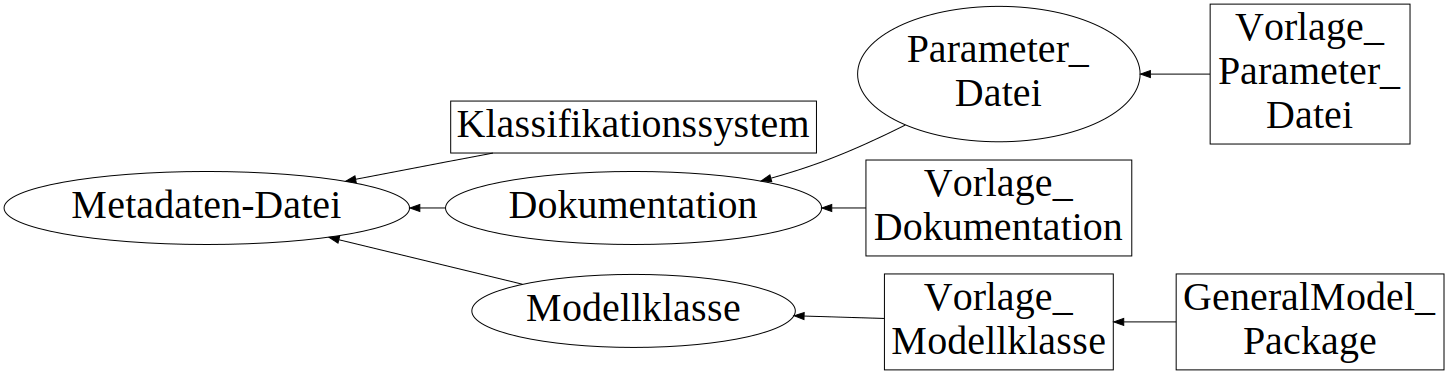
\includegraphics[width=1\linewidth]{Katalogstruktur}
	\caption[Katalogstruktur]{Katalogstruktur. Elemente in Ellipsen existieren individuell für jedes Modell. Elemente in Rechtecken existieren genau ein einziges Mal im Katalog.}
	\label{fig:Katalogstruktur}
\end{figure}
%
Das \textit{Klassifikationssystem} ist eine Übersicht der Modelleigenschaften und deren Beziehungen untereinander. Die Einträge in dem Feld für die Modelleigenschaften in der Metadaten-Datei (\textit{tag\_list}) sind bevorzugt Namen von Kategorieknoten aus dem KS. Es sorgt für eine einheitliche Namensgebung der Modelleigenschaften (s. Anforderung \ref{A.Modelleigenschaften}). 

Das Python Package \textit{GenericModel} stellt die Python-Klasse \textit{GenericModel} zur Verfügung, von der alle Modellklassen der implementierten Modelle erben. Sie stellt Variablen und Methoden bereit, die alle Modellklassen gemeinsam haben.

Die \textit{Metadaten-Datei} ist eine Datei im YAML-Format, die Felder für Informationen enthält, in die Informationen des zugehörigen Modells eingetragen werden können. Es gibt Felder für Informationen \dots 
\begin{itemize}[label=$\bullet$]
	\item über das Modell (Modellname, Kurzbeschreibung, Modelleigenschaften, Dateinamen eventueller Modellbilder)
	\item für eine Umsetzung des Kataloges als Datenbank (Key, Predecessor-Key, Implementation-Key)
	\item anderer Art (Modellersteller, Erstellungsdatum, Liste der Bearbeiter, Externe Referenzen)
\end{itemize}
Das Konzept und die Umsetzung der Metadaten-Datei basieren auf \cite{KNHE20b}. 
% Noch schreiben welche Informationen im aktuellen Stand gegeben werden?

Die \textit{Modelldokumentation} ist die textuelle Notation des Modells. Sie wird im \LaTeX-Format geschrieben. Nach jeder Bearbeitung wird die PDF-Datei aus der \LaTeX-Datei erzeugt. 

Die \textit{Parameter-Datei} ist eine Python-Datei. Diese enthält beispielhafte Parameterwerte für das Modell. Das Ausführen der Datei erzeugt eine Tabelle mit den beispielhaften Parameterwerten im \LaTeX-Format und speichert diese in einer Datei Namens \textit{parameters.tex} im Ordner der Modelldokumentation ab. Außerdem stellt Sie eine Methode für die implementierte Modellklasse bereit, welche die Parameter des Modells als Rückgabewert hat.

Die implementierte \textit{Modellklasse} ist eine Python-Datei, welche das Modell als Python-Klasse enthält. 

Die \textit{Vorlagen} für die Metadaten-Datei, die Parameter-Datei, die Modelldokumentation und -implementation sind Dateien, welche den Arbeitsaufwand für das Anlegen neuer Modelle verringern sollen(siehe Entscheidung \ref{E.Vorlagen}). Die repetitiven Elemente für die entsprechenden Dateien sind in den Vorlagen schon vorhanden, sodass nur die Modellspezifischen Elemente neu geschrieben werden müssen. Die Verwendung der Vorlagen stellt außerdem eine einheitliche Struktur der Dateien sicher.

Die Ordnerstruktur des Kataloges liegt in einem Git-Repositorium\footnote{Der Katalog hat kein eigenes Repository, sondern liegt aktuell im Git-Repository dieser Studienarbeit. Deshalb wird an dieser Stelle kein Link zur Verfügung gestellt.} (s. Entscheidung \ref{E.Git}).  

\begin{figure}[H]
	\centering
	\begin{adjustbox}{padding=15pt 0pt 0pt 0pt, fbox}
		\begin{lstlisting}[basicstyle=\footnotesize, extendedchars=false]
Katalogue_of_dynamical_and_control_Systems
+---01_Models
|   |   Model_Documentation_Template.tex
|   |   Model_Template.yml 
|   |
|   +---Model_1
|   |       metadata.yml
|   |       Model_1_Documentation.tex
|   |       Model_1_Documentation.pdf	
|   |
|   +---Model_2
|   ...
+---02_Implementations
|   |   Model_Class_template.py
|   |   parameters_template.py
|   |             
|   +---Model_1
|   |       Model_1_Class.py
|   |       Model_1_paramters.py
|   |       (optional für Git) Model_1_Test.py
|   |
|   +---Model_2
|   ...
+---03_GenericModel_package
\---04_Classification_System

		\end{lstlisting}
	\end{adjustbox}
	\caption[Ordnerstruktur des Kataloges]{Ordnerstruktur des Git Repositoriums des Kataloges mit schematischer Inhaltsdarstellung des Modell- und Implementationsordners.}
	\label{fig:Ordnerstruktur}
\end{figure}

% =================================================
% ------------- Klassifikationssystem -------------
% =================================================
\section{Klassifikationssystem}
\label{Ch:Ergebnisse:Sec:KS}
Das \textit{Klassifikationssystem (KS)} stellt eine Wissensrepräsentation dar. Es lehnt stark an die in \cite{KNHE20a} eingeführte \textit{OCSE} an, von der es sich insofern unterscheidet, dass im KS nur die Teilbereiche des Wissens der Mathematik, Regelungs- und Steuerungstheorie enthalten sind, die sich auf regelungstechnische Systeme und Modelle beziehen. Die im KS verwendeten Bezeichnungen sollen in den Metadaten-Dateien der Modelle bevorzugt verwendet werden. \\
Es ist anzumerken, dass das KS keine vollständige Wissensrepräsentation darstellt, da diese nur mit sehr hohem Aufwand erstellbar ist. Zum Einen, weil das potenziell darzustellende Wissen sehr umfangreich ist und zum Anderen, weil aus Sicht des Autors eine vollständige Darstellung des beabsichtigten Wissens, aufgrund der dynamischen Erweiterung des Wissens durch neue Entdeckungen und der daraus ableitbaren Unvollständigkeit des bestehenden Wissens, nicht existiert. In jedem Fall ist klar, dass im Rahmen dieser Studienarbeit nur ein Teilbereich des beabsichtigten Wissens abgebildet werden kann. 

Bei einem konkreten Modell im Katalog finden sich die Einträge des KS im Informationsfeld \textit{tag\_list} der Metadaten-Datei wieder. In diesem Informationsfeld werden die Modelleigenschaften und dessen Werte notiert. Für die Einträge in der \textit{tag\_list} gilt eine Open-World Annahme. Wenn eine Eigenschaft nicht in der \textit{tag\_list} enthalten ist, dann enthält der Katalog keine Aussage darüber, ob das Modell die Eigenschaft besitzt oder nicht.

Das KS besteht aktuell aus 90 Knoten. \autoref{fig:KS_Snippet} zeigt einen Ausschnitt des KS.

% BILD: Ausschnitt KS, aus Modelleigenschaften
% ============================================
\begin{figure}[bh]
	\centering
	\includegraphics[trim=0 680.7 109.5 0, clip, width=0.9\linewidth]{KS_Snippet}
	\caption{Ausschnitt des Klassifikationssystems}
	\label{fig:KS_Snippet}
\end{figure}

% =============================================================
% ------------- Aufbau des Klassifikationssystems -------------
% =============================================================
\subsection{Aufbau des Klassifikationssystems}
\label{Ch:Ergebniss:Sec:KS:SubSec:Aufbau}
Das KS ist ein Semantisches Netz (s. \autoref{E.KS_SemantischesNetz}), welches durch einen gerichteten, kreisfreien Graphen repräsentiert wird. Es gibt folgende Knotentypen: Kategorie-, Werte-, und Wertetypknoten. 
Die Kanten zeigen Beziehungen zwischen den Knoten des KS auf, die durch die Kantenbeschriftungen spezifiziert werden. Es gibt folgende Kantennamen: \glqq is a\grqq, \glqq value of\grqq und \glqq type of\grqq.. Der Kantenname kennzeichnet zudem den Knotentyp des Startknotens der Kante. Jeder Endknoten einer Kante ist ein Kategorieknoten. Die Beziehung zwischen Knotentypen und Kantennamen wird in \autoref{table:KS_KantenUndKnoten} gezeigt.

% TABELLE: Kantennamen - Knotentypen Beziehung
% ============================================
\begin{table}[H]
	\centering
	\begin{tabular}{l|c|l}
		Startknotentyp & Kantenname & Endknotentyp \\ \hline
		Kategorieknoten & is a & Kategorieknoten \\
		Werteknoten & value of & Kategorieknoten \\
		Wertetypknoten & type of & Kategorieknoten 
	\end{tabular}
	\caption{Beziehung zwischen Kantennamen und Knotentypen}
	\label{table:KS_KantenUndKnoten}
\end{table}
%
Die Kategorieknoten, außer der Ursprungsknoten und die Knoten der Hauptkategorien, können als Modelleigenschaften interpretiert werden. \\
Die Kategorieknoten im KS werden durch ihren eindeutigen Namen identifiziert (s. \ref{E.KS_Namensgebung}).\\
Jeder Knoten $k$, außer der Ursprungsknoten, ist entlang eines gerichteten Pfades $P(k)$ mit dem Ursprungsknoten verbunden. Wird einem Modell ein Knoten $k_i$ des KS als Modellattribut zugewiesen, dann hat das Modell auch alle Knoten, außer die Knoten der Ursprungs -und Hauptkategorie(-n), entlang des gerichteten Pfades $P(k_i)$ als Modellattribut. Aus diesem Grund wird in der \textit{tag\_list} der Metadaten-Datei immer nur die spezifischste Eigenschaft eines Pfades angegeben. % Beispiel?

Der Ursprungsknoten \textit{Property\_Of\_Classification\_System} hat die drei Unterkategorien \textit{Property\_Of\_Mathematical\_Representation}, \textit{Model\_Attribute} und \textit{Usage\_Area}. Die Unterkategorien des Ursprungsknoten werden im KS als Hauptkategorien bezeichnet, die jeweils verschiedene Teilmengen von Modellattributen enthalten. Die Hauptkategorien werden wie folgt beschrieben.

\textbf{Eigenschaften der mathematischen Repräsentation}: \\
Umfasst Eigenschaften der mathematischen Repräsentation des Modells.   % ... die aus der math. Rep. direkt hervor gehen. --> Äquivalenzbegriff von Willems

\textbf{Modelleigenschaften}: \\ % Eigenschaften unabhängig von Darstellungsform eines äquivalenten Systems
Umfasst Eigenschaften, die aus der mathematischen Repräsentation mit Methoden der Regelungstechnik abgeleitet werden.

\textbf{Anwendungsgebiete}: \\
Umfasst Aufgabentypen und Anwendungsbereiche, in denen die Modelle häufig genutzt werden.

In \autoref{Ch:Vorbetrachtung:Sec:SystemeModelle} wurde erwähnt, dass ein Modell mehrere mathematische Repräsentationen haben kann. Dieser Aspekt führt auf den Begriff der \textit{Äquivalenz} zweier mathematischer Modelle. Zwei mathematische Modelle heißen \textit{äquivalent}, wenn beide die gleiche Menge an Trajektorien für ihre externen Variablen zulassen\footnote{vgl. \cite[S. 34]{SCH89}}. Oder einfacher, wenn beide Modelle das gleiche dynamische Verhalten aufweisen. Das Modell eines Systems kann durch eine Menge äquivalenter mathematischer Modelle repräsentiert werden. Der Unterschied zwischen den Hauptkategorien \textit{Eigenschaft der mathematischen Repräsentation} und \textit{Modelleigenschaften} liegt darin, dass die Elemente eine Menge äquivalenter mathematischer Modelle die gleichen Modelleigenschaften haben, sich aber in ihrer mathematischen Repräsentation unterscheiden.

% ===========================================================================
% ------------- Technische Umsetzung des Klassifikationssystems -------------
% ===========================================================================
\subsection{Technische Umsetzung des Klassifikationssystems}
\label{Ch:Ergebnisse:Sec:KS:SubSec:TechUmsetzung}
Das KS wird technisch durch vier Dateien im YAML-Format realisiert, welche folgende Namen haben: \textit{KS\_Tree\_main}, \textit{KS\_Tree\_Math\_Representation}, \textit{KS\_Tree\_Model\_Attributes} und \textit{KS\_Tree\_Usage\_Area}. Die Datei \textit{KS\_Tree\_main} enthält die \textit{Informationsblöcke (IB)} zu dem Ursprungsknoten und den Knoten der Hauptkategorien. Die restlichen drei Dateien enthalten jeweils die Informationsblöcke zu den Knoten der Unterkategorien der Hauptkategorien. \\ 
Ein IB enthält alle Informationen zu genau einem Knoten des KS. Jeder IB in den YAML-Dateien ist ein Mapping. Ein Mapping, gekennzeichnet durch einen Doppelpunkt, setzt einen Schlüssel mit genau einen Wert in Beziehung. Das \textit{dictionary} ist das Python-Äquivalent zu einem Mapping. In jedem IB ist der Name des Knotens der Schlüssel und eine Sequenz ist der Wert. Eine Sequenz ist in YAML eine Folge von Zeilen, die mit einem Strich beginnen und der Inhalt der Zeile stellt einen Eintrag der Sequenz dar. \textit{List} und \textit{tuple} sind die Python-Äquivalente zur Sequenz. Jeder Eintrag der Sequenz steht für ein Attribut des Knotens und ist wiederum ein Mapping, dessen Schlüssel der Attributsname und dessen Wert der Attributswert ist. Die IB\grq s sind durch eine Leerzeile voneinander getrennt. Die \autoref{fig:IBs} zeigt einige IB\grq s aus der Datei \textit{KS\_Tree\_Math\_Representation}.

% BILD: Informationsblöcke
%=========================
\begin{figure}[b]
	\centering
	\begin{adjustbox}{padding=15pt 0pt 0pt 0pt, fbox}
	\begin{lstlisting}[basicstyle=\footnotesize]
General_Function:
	- Type: boolean
	- Pre_Node: Property_Of_Mathematical_Representation
	- Edge_Name: is a

DAE: 
	- Type: boolean
	- Pre_Node: General_Function
	- Edge_Name: is a
	\end{lstlisting}
	\end{adjustbox}
	\caption{Informationsblöcke des KS}
	\label{fig:IBs}
\end{figure}

Eine Kante wird durch die Elemente \textit{Pre\_Node} und \textit{Edge\_Name} definiert. Diese stehen jeweils als Einträge in der Sequenz des Informationsblocks des Startknotens der Kante.

Zusätzlich gibt es das Python-Skript \textit{KS\_Create\_Graph}, welches die YAML-Dateien mit Hilfe des Packages \textit{pyyaml}\footnote{Pyyaml-Package: \url{https://pyyaml.org/wiki/PyYAMLDocumentation}} einliest. Zudem erzeugt es einen gerichteten Graphen des Python-Packages \textit{networkx}\footnote{Networkx Package: \url{https://networkx.org/documentation/stable/index.html}} und zeichnet den Subgraphen, der nur die Kategorieknoten enthält mit dem Python-Package \textit{nxv}\footnote{Nxv-Package: \url{https://nxv.readthedocs.io/en/latest/index.html}} in eine Bilddatei.

Ein gerichteter Graph des networkx-Packages besteht aus einer Menge von Knoten und Kanten. Zu jedem Knoten und jeder Kante kann eine beliebig große Menge individuell benannter Attribute hinzugefügt werden. So werden z.\,B. die Kantennamen der entsprechenden Kante als Attribut hinzugefügt. Die Wertetypknoten sind als Attribut eines Kategorieknotens implementiert. Diese Umsetzung des implementierten Graphen ist aus technischer Sicht sinnvoll, da die Information über die Attribute eines Knotens so intuitiver zu erreichen sind. Es soll hier jedoch erwähnt werden, das diese Implementierung von einer korrekten Darstellung des KS als Semantisches Netz abweicht, da Kategorieknoten nur explizit als Knoten aufgeführte Attribute besitzen. Für eine formal korrekte Implementierung des KS als Semantisches Netz müssten Knoten, welche die Attribute einer Kategorie darstellen, auch explizit als Knoten angelegt werden.\\
Die gewählte Implementierung des KS ist einfach erweiterbar und bearbeitbar. Eine Veränderung im Umfang des KS, also das Hinzufügen neuer Knoten zum KS oder das entfernen von Knoten aus dem KS, wird in der Implementierung durch schreiben neuer IB\grq s oder entfernen bestehender IB\grq s erreicht. Sollen neue Knotentypen zum KS hinzugefügt werden wie z.\,B. Referenzknoten, welche eine Referenz zur Definition der Kategorie enthalten würden, so werden diese als neuer Eintrag zu den Sequenzen der IB\grq s hinzugefügt.

%TODO: Vllt eher in Ausblick?
Die Implementierung des KS ist auch relativ einfach für eine potenzielle Integration einer Suchfunktion zu öffnen, indem zu dem Python-Skript \textit{KS\_Create\_Graph} eine Methode hinzugefügt wird, welche die networkx-Graphen des KS als Rückgabewert liefert.  
% Networkx-Graphen vom Funktionsumfang potenziell als vollständige maschinelle lesbare Repräsentation des KS und dessen Anwendungen auf die Modelle verwendbar

% ===============================================
% ------------- Modelldokumentation -------------
% ===============================================
\section{Modelldokumentation}
\label{Ch:Ergebnisse:Sec:Dokumentation}
Die Modelldokumentation enthält die textuelle Notation des Modells in einer Datei im \LaTeX-Format. Die Dokumentation besteht aus den Abschnitten: \textit{Nomenklatur}, \textit{Modellgleichungen}, \textit{Herleitung und Erklärungen} und \textit{Referenzen}. Der Abschnitt \textit{Herleitung und Erklärung} ist optional.

\textbf{Nomenklatur}:\\
Die Nomenklatur enthält alle in der Dokumentation genutzten Variablen und eine Beschreibung, für welche Größen diese stehen. Die Nomenklatur ist aufgeteilt in die Sektionen \textit{Nomenklatur für die Modellgleichungen} und \textit{Nomenklatur für die Herleitung}. Die Nomenklatur für die Modellgleichungen enthält die Variablen, die im gleichnamigen Abschnitt verwendet werden und muss in jeder Dokumentation enthalten sein. Die Nomenklatur für die Herleitung enthält alle Variablen, die für den Abschnitt \textit{Herleitung und Erklärung} genutzt werden, bis auf die Variablen die in der Sektion \textit{Nomenklatur für die Modellgleichungen} schon enthalten sind. Die Nomenklatur für die Herleitung ist nur zu schreiben, wenn der Abschnitt \textit{Herleitung und Erklärung} existiert. \autoref{fig:BspDok_Nomenclature} zeigt die Nomenklatur zum Model des Hochsetzstellers.

% BILD: Dokumentation Nomenklatur
% ===============================
\begin{figure}[H]
	\centering
	\fbox{\includegraphics[trim=120 520 120 110, clip, width=0.9\linewidth]{Boost_Converter_Documentation}}
	\caption[Beispiel zur Nomenklatur der Dokumentation]{Nomenklatur aus der Dokumentation zum Hochsetzsteller (Boost-Converter)}
	\label{fig:BspDok_Nomenclature}
\end{figure}
%
\textbf{Modellgleichungen}:\\
Der Abschnitt \textit{Modellgleichungen} besteht aus einer formalisierten Darstellung der Modellgleichungen und weiteren Sektionen, die anschließend benannt werden. Die formalisierte Darstellung der Modellgleichungen besteht aus drei Teilen:  
\begin{itemize}[label=$\bullet$]
	\item einer Zuordnung der Variablen zum generalisierten Zustands-, Eingangs- und (optional) Ausgangsvektor
	\item einem Gleichungssystem von Differentialgleichungen erster Ordnung (s. \ref{E.Textdok}), das die generalisierten Zustands- und Eingangsvariablen verwendet
	\item der Benennung, welche Variablen Parameter sind
\end{itemize} 
Der Abschnitt der Modellgleichungen aus der Dokumentation des Hochsetzstellers ist in \autoref{fig:BspDok_ModelEquations} zu sehen.

% BILD: Dokumentation Modellgleichungen
% =====================================
\begin{figure}[H]
	\centering
	\fbox{\includegraphics[trim=120 300 120 340, clip, width=0.9\linewidth]{Boost_Converter_Documentation}}
	\caption[Beispiel der Gleichungen der Dokumentation]{Gleichungen aus der Dokumentation zum Hochsetzsteller (Boost-Converter)\protect\footnotemark}
	\label{fig:BspDok_ModelEquations}
\end{figure}
\footnotetext{Modell stammt aus \cite[Abschnitt 1.3]{ROEB17}}
%
Die weiteren Sektionen sind recht frei gestaltbar und sollen weitere nützliche Informationen zu dem Modell liefern. Aktuell sind in der Vorlage nur die Sektionen \textit{Annahmen} und \textit{Beispielhafte Parameterwerte} explizit formuliert. Weitere Sektionen können vom Ersteller des Modells nach eigener, subjektiver Einschätzung der Sinnhaftigkeit hinzugefügt werden. Denkbar wäre, angenommen es handelt sich um ein flaches Modell, z.\,B. ein Abschnitt, der flache Ausgänge angibt. Die Sektion \textit{Beispielhafte Parameterwerte} ist als einzige unter den weiteren Sektionen zwingend zu füllen. Dies geschieht mehr oder weniger automatisch, da die Datei \textit{paramters.tex}, die durch die \textit{Parameter-Datei} erstellt wird, dafür eingebunden wird.

\textbf{Herleitung und Erklärungen}:\\
Dieser Abschnitt ist für die Dokumentation optional. Er soll die Möglichkeit bieten, die Herleitung des Modells zu beschreiben oder weitere aus Sicht des Modellerstellers sinnvolle Erklärungen zu liefern.

\textbf{Referenzen}:\\
Enthält die Referenzen, die für die Erstellung der Modelldokumentation verwendet wurden.

Aus der \LaTeX-Datei der Modelldokumentation wird eine für Menschen gut lesbare PDF-Datei erzeugt. 

% =================================================
% ------------- Modellimplementation  -------------
% =================================================
\section{Modellimplementation}
\label{Ch:Ergebnisse:Sec:Implementation}
Modelle des Kataloges werden in Form einer Python-Klasse implementiert. Bei Initialisierung eines Objektes der Modellklasse können dem Konstruktor die Zustandsdimension, eine Eingangsfunktion und ein Parametervektor übergeben werden. Alle diese Variablen haben Standardwerte. Jede Modellklasse bezieht ein Standardset von Parameterwerten aus der \textit{Parameter-Datei} (die Standardparameter sind also identisch mit den beispielhaften Parameterwerten aus der Dokumentation) und hat eine Standardfunktion für die Modelleingänge bzw. die Eingangsfunktion integriert.\\ 
Ein Modell kann also einfach über ein selbst erstelltes Python-Skript simuliert werden (vgl. \ref{A.Implementierung}), indem eine Objekt der Modellklasse erzeugt wird, ein Startvektor für den Modellzustand definiert wird und anschließend das Modell mit einer geeigneten Methode (z.\,B. \textit{solve\_ivp} des Python-Packages \textit{scipy}\footnote{SciPy-Package: \url{https://www.scipy.org/}}) simuliert wird. Die Methode \textit{get\_rhs\_func}\footnote{\textit{rhs} steht für \textit{right hand side}} der Modellklasse stellt die dafür benötigte Python-Funktion zur Verfügung.

Die Parameter und die Eingangsfunktion eines Modellobjektes können nach Initialisierung mit den Methoden \textit{set\_parameters} und \textit{set\_input\_func} geändert werden. Die Zustandsdimension ist nur bei Initialisierung einstellbar und das auch nur bei Modellen, deren Zustandsdimension nicht festgelegt ist (z.\,B. beim N-Fach-Integrator).\\
Die Methode \textit{get\_rhs\_symbolic} liefert die symbolischen Modellgleichungen als Rückgabewert. Zur Implementierung der symbolischen Gleichungen wird das Python-Package \textit{sympy}\footnote{SymPy-Package: \url{https://www.sympy.org/en/index.html}} verwendet.

%Obsoloter Absatz?
Jede Modellklasse erbt von der Klasse \textit{GenericModel}, welche eine Menge von Methoden und Variablen definiert, die jede Modellklasse haben muss. Die Methoden, die nicht für jede individuelle Modellklasse angepasst werden müssen, sind in der Klasse \textit{GenericModel} bereits implementiert.\\
Innerhalb einer Modellklasse sind nur die symbolischen Gleichungen als Code geschrieben. Die Umwandlung in die numerische Form erfolgt in der Methode \textit{get\_rhs\_func} mit der Methode \textit{lambdify} des Sympy-Packages.
% Hinweis das bei Codesyntax versucht wurde nach PEP8 zu arbeiten?

Mittels der aktuellen Vorlagen können nur Modelle, deren Verhalten durch ein gewöhnliches Differentialgleichungssystem erster Ordnung beschrieben wird, implementiert werden.

% ==============================================
% ------------- Vorhandene Modelle -------------
% ==============================================
\section{Vorhandene Modelle}
\label{Ch:Ergebnisse:Sec:Modelle}
Die aktuell im Katalog enthaltenden Modelle sind in \autoref{table:AktuelleModelle} aufgelistet. 

% TABELLE: Aktuelle Modelle
% =========================
\begin{table}[H]
	\begin{tabular}{r|l|c|c}
		Nr & \multicolumn{1}{c|}{Modellname} & Modelldimension & Implementiert? \\ \hline
		1 & Hochsetzsteller & 2 & Nein \\
		2 & Brockett-Integrator & 3 & Ja \\
		3 & DC-DC Tiefsetzsteller & 2 & Nein \\
		4 & Heisenberg-Flugrad & 3 & Nein \\
		5 & Kapitzas Pendel & 2 & Ja \\
		6 & Lorenz Attraktor & 3 & Ja \\
		7 & MMC\tablefootnote{Modular Multilevel Converter} & 8 & Nein \\
		8 & N-Fach Integrator & n & Ja \\
		9 & PVTOL mit 2 Kräften\tablefootnote{Planar Vertical Takeoff and Landing [Vehicle] (dt. Senkrechtstarter)} & 6 & Ja \\
		10 & Rössler Attraktor 1979a & 3 & Ja \\
		11 & Stabiles PT$_{n}$-Glied & n & Ja
	\end{tabular}
	\caption{Modelle des Kataloges}
	\label{table:AktuelleModelle}
\end{table} 

% ==============================================
% ------------- Katalogerweiterung -------------
% ==============================================
\section{Katalogerweiterung}
\label{Ch:Ergebnisse:Sec:Erweiterung}
Die letzte Anforderung an den Katalog war, das dieser erweiterbar sein soll (Anforderung \ref{A.Erweiterbarkeit}). In diesem Abschnitt wird beschrieben, welche Schritte für die Erweiterung des Kataloges nötig sind. 

Der Katalog wird über das Hinzufügen neuer Modelle erweitert.

Es werden folgende Annahmen getroffen:
\begin{enumerate}
	\item Die Recherche für das hinzuzufügende Modell ist abgeschlossen. Die nötigen Informationen zu dem Modell wie Modellgleichungen, beispielhafte Parameterwerte, Beschreibung der Variablen und die dazugehörigen Referenzen sind also schon bekannt.
	\item Der Modellersteller hat sich mit der Ordnerstruktur des Kataloges vertraut gemacht.
\end{enumerate}

Für das Anlegen eines neuen Modells im Katalog sind folgende Schritte notwendig:
\begin{enumerate}
	\item Git installieren und das Git-Repositorium (siehe \ref{E.Git}) des Kataloges herunterladen um eine lokale Kopie des Kataloges und der Vorlagen (siehe \autoref{Ch:Ergebnisse:Sec:Struktur}) zu erhalten.
	\item Anlegen und benennen eines neuen Modell- und Implementationsordners.
	\item Erstellen der \textit{Metadaten-Datei} im Modellordner mithilfe der Vorlage und Umbenennung dieser in \textit{metadata.yml}.
	\item Erstellen der \textit{Modelldokumentation} im Modellordner mithilfe der Vorlage.
	\begin{enumerate}[label=\textbf{Anmerkung \arabic*}:, wide=0pt, leftmargin=*]
		\item Die Vorlage stellt aktuell nur eine einheitliche Notation für gewöhnliche Differentialgleichungssysteme erster Ordnung zur Verfügung. Modelle, deren Modellgleichungen in ein gewöhnliches Differentialgleichungssystem erster Ordnung transformierbar sind, müssen in ein solches transformiert werden.
		\item Für Modelle, deren Modellgleichungen nicht in ein gewöhnliches Differentialgleichungssystem erster Ordnung transformierbar sind, gibt es noch keine festgelegte Notationsvorgabe.
	\end{enumerate}
	\item Erstellen der \textit{Parameter-Datei} im Implementationsordner mithilfe der Vorlage und ausführen\footnote{Zur Erinnerung: Die Parameter-Datei ist ein Python Skript.} dieser.
	\item Die PDF-Datei der Modelldokumentation erzeugen.
	\item (optional, siehe \ref{E.ImplementierungOptional}) Erstellen der \textit{Modellklasse} im Implementationsordner mithilfe der Vorlage.
	\begin{itemize}[label=\textbf{Anmerkung}:, wide=0pt, leftmargin=*]
		\item Aktuell können nur Modelle, die durch ein gewöhnliches Differentialgleichungssystem erster Ordnung beschrieben werden, mithilfe der Vorlage implementiert werden.
	\end{itemize}
	\item Pull-Request ausführen.
\end{enumerate}







% Kapitel 4: Zusammenfassung und Ausblick
% 4.1 Übersicht zu aktuellem Funktions- und Modellumfang
% 4.2 Ausblick
\chapter{Zusammenfassung und Ausblick}
\section{Übersicht zu aktuellem Funktions- und Modellumfang} 
Inhalt:\\
Aktueller Stand bzgl. Modellumfang und möglicher Modellkomplexität --> Problem mit komplexen Größen \\
Aktuelle Vorlagen und Limitierungen, Aufwandseinschätzung für das Hinzufügen neuer Modelle \\

\section{Ausblick} 
Inhalt: \\
Was noch denkbar/wünschenswert/möglich wäre bzgl. Funktionsumfang \\
Versionsverwaltung, Ideen/Konzept zur Öffnung für breite(re) Nutzerschaft(Mögliche Vorlage: ACKRep, aber evtl. Orientierung auch an anderen Nutzer basierten Datenbanken (Wiki-like))\\ 
Abfragbare KS Implementierung via networkx-Package die weitere Informationen zu Einträgen des KS enthält (kurze Beschreibung, Referenz bzgl. Bedeutung --> Umsetzung mit .bib Datei und Verweis auf Kürzel + ggf. Seitenangabe etc.)\\
Suchfunktion \\
Automatische Erstellung einer Übersicht aller der enthaltenen Modelle (ist Verknüpft mit Suchfunktion?)


% ==================================
% Literaturverzeichnis
% ==================================

% Ein Literatureintrag, der nicht referenziert wird, aber im Verzeichnis erscheinen soll
\nocite{ROE79}

% Literaturverzeichnis ausgeben
\printbibliography

\end{document}


%%% Local Variables:
%%% mode: latex
%%% TeX-master: t
%%% End:
